\chapter[Membrane potential heterogeneity at the cellular level]{Membrane potential heterogeneity at the cellular level: mother-bud asymmetry of mitochondrial function in budding yeast}\label{ch:six}
\clearpage
\section{Introduction}
Eukaryotic cells exhibit cell polarity, i.e. spatial heterogeneity in the structure and function of cellular components such as the cytoskeleton, organelles and cell surfaces. Cell polarity results from asymmetric distribution and organization of cellular components and function within the cell. Well known examples are the apical and basolateral plasma membrane domains in epithelial cells and the dendrite and axon terminals seen at the synapses of neurons. The life cycle of organisms exhibit polarity in the form of asymmetric cell division. Young individuals are born with low levels of damaged proteins that is mostly independent of the age of their parents. This is thought to be crucial to maintain healthy germline cells at the expense of somatic cells ('disposable soma theory', \cite{kirkwood_evolution_1979}.

Budding yeast experience polarized cell growth at several stages during its life cycle. For example haploid cells exposed to a pheromone from another cell of the opposite mating type arrest cell growth in G1 and form projections towards the other cell \cite{madden_cell_1998}. While mating is a distinct transition in the life cycle of budding yeast, for this thesis we are only interested in their mitotic life cycle. Budding yeast cells undergo cell proliferation where the original mother cell gives rise to a bud/daughter cell with an entirely new cell surface. While budding yeast does not have a germline/somatic cell distinction, they do display age related changes in cellular function and fitness. Mother cells do not divide forever, they stop after around 20--25 divisions and then enter a short postreplicative state before lysis \cite{longo_replicative_2012}. The number of times the mother cell can divide is known as its replicative life span. As it ages, the mother cell exhibits accumulation of oxidatively damaged proteins and extrachromosomal rDNA circles \cite{aguilaniu_asymmetric_2003}, impaired mitochondria \cite{lai_mutation_2002} and eventually loses the ability to undergo further cell division \cite{laun_aged_2001}. However daughter cells are born with full replicative potential \cite{steinkraus_replicative_2008} and much lower levels of oxidative stress \cite{aguilaniu_asymmetric_2003}. Oxidative damage is thought to contribute to age related decline in mitochondrial and cellular function \cite{huang_role_2004,lai_mutation_2002}.

There is emerging evidence for the existence of a mitochondrial quality control mechanism via fission and fusion to segregate healthy mitochondria and that buds preferentially inherit these mitochondria during cell division \cite{klinger_quantitation_2010,mcfaline-figueroa_mitochondrial_2011}. An early study noted a reduced level of mitochondrial membrane potential (ΔΨ) in older populations of budding yeast cells using flow cytometry \cite{lai_mutation_2002}. This study was done using a method that lacks single cell resolution level, and hence cannot answer how functional asymmetry is distributed within the cell. A study by Pon et al. \cite{mcfaline-figueroa_mitochondrial_2011} showed evidence of an intracellular asymmetry of function in budding yeast at single cell resolution level. They quantified levels of oxidative redox potential using a mitochondrial matrix targeted fluorescent protein marker (roGFP1) and also superoxide levels by staining with dihydroethidium (DHE). They found that mother cells retained mitochondria with a lower ratio of reduced to oxidized roGFP1 and higher superoxide levels compared to buds. They also showed that the ratio of reduced to oxidized roGFP1 in mother and bud cells decreased with replicative age, meaning that mitochondria in old cells were more oxidized .

What the above studies lacked was that there was no analysis of the spatial distribution of function in mitochondrial networks along the mother-bud cell axis. This means that previous studies did not quantify the distribution of a functional marker at specific regions along this axis that might be important to the cell cycle. For example, the bud neck is believed to be a bottleneck for movement of all cargoes into the bud \cite{vevea_inheritance_2014} and it would be interesting therefore to see if mitochondrial quality around this region could impact bud growth. Using the methods developed in \Fref{ch:two}, we extended the analysis of functional heterogeneity of mitochondria at the cellular level using the distribution of ΔΨ along an axis that represents the polarity of the mother-bud cell axis. We show for the first time how ΔΨ is distributed along this axis and provides a quantitative analysis of how this ΔΨ distribution varies with budding progression.
\section{Materials and Methods}
\subsection{Picking of points to define the mother-bud axis}
We used the open-source Mayavi 3D visualization software (\url{http://code.enthought.com/projects/mayavi/}) to render in 3D the mitochondrial network skeleton based on the outputs from MitoGraph v2.0. Mayavi has convenient function wrappers in Python for handling VTK objects and makes it easier to write interactive software for the cell picking procedures described below.

The cell surfaces (yellow ellipses) shown in \Fref{fig:coors} were drawn using the Mayavi's Parametric Surface function. The major and minor axis length, center coordinate and angle of the ellipse was obtained via an ImageJ ellipse fit of a hand traced ROI of the brightfield data of the actual cell, as detailed in \fref{sec:ROI}. The surfaces shown represent the 3D rendering of that ellipse fit. Additionally, it was often necessary to center the cell surfaces in the $z-$axis. This was because the focal slice position used to trace the brightfield image was often not aligned with the $z-$axis midpoint of the mitochondrial skeleton (which is based on MitoGraph v2.0's coordinate outputs). This would often result in the skeleton 'jutting out' in the $z-$axis from the cell surface (\Fref{fig:caveatA}). Centering was done via another mouse callback function by iteratively picking a position in the skeleton (magenta dot in the figure) that resulted in full enclosure of the skeleton by the cell surface.

To define the mother-bud axis, we picked three points; the base, tip and neck points on the cell surfaces via a mouse callback function (a function invoked when a mouse button was pressed). The base and tip represent the ends of the cell surfaces on the mother side and the bud side respectively. For the picking of the neck point, the intersection between mother and bud was estimated by taking the mid point of the intersection between the mother and bud surfaces (\Fref{fig:caveatB}). Care was also taken to pick the extreme ends of the cell surface and not the skeleton (\Fref{fig:caveatC}, blue and green dots). This was important because the mitochondrial skeleton was not always fully distributed at the ends of the cell surface, especially in cells with low amount density of mitochondria. Picking the points on the surface allows us to obtain correct correct localization of the mother-bud axis.
%
\begin{figure}[htp]
	\centering
    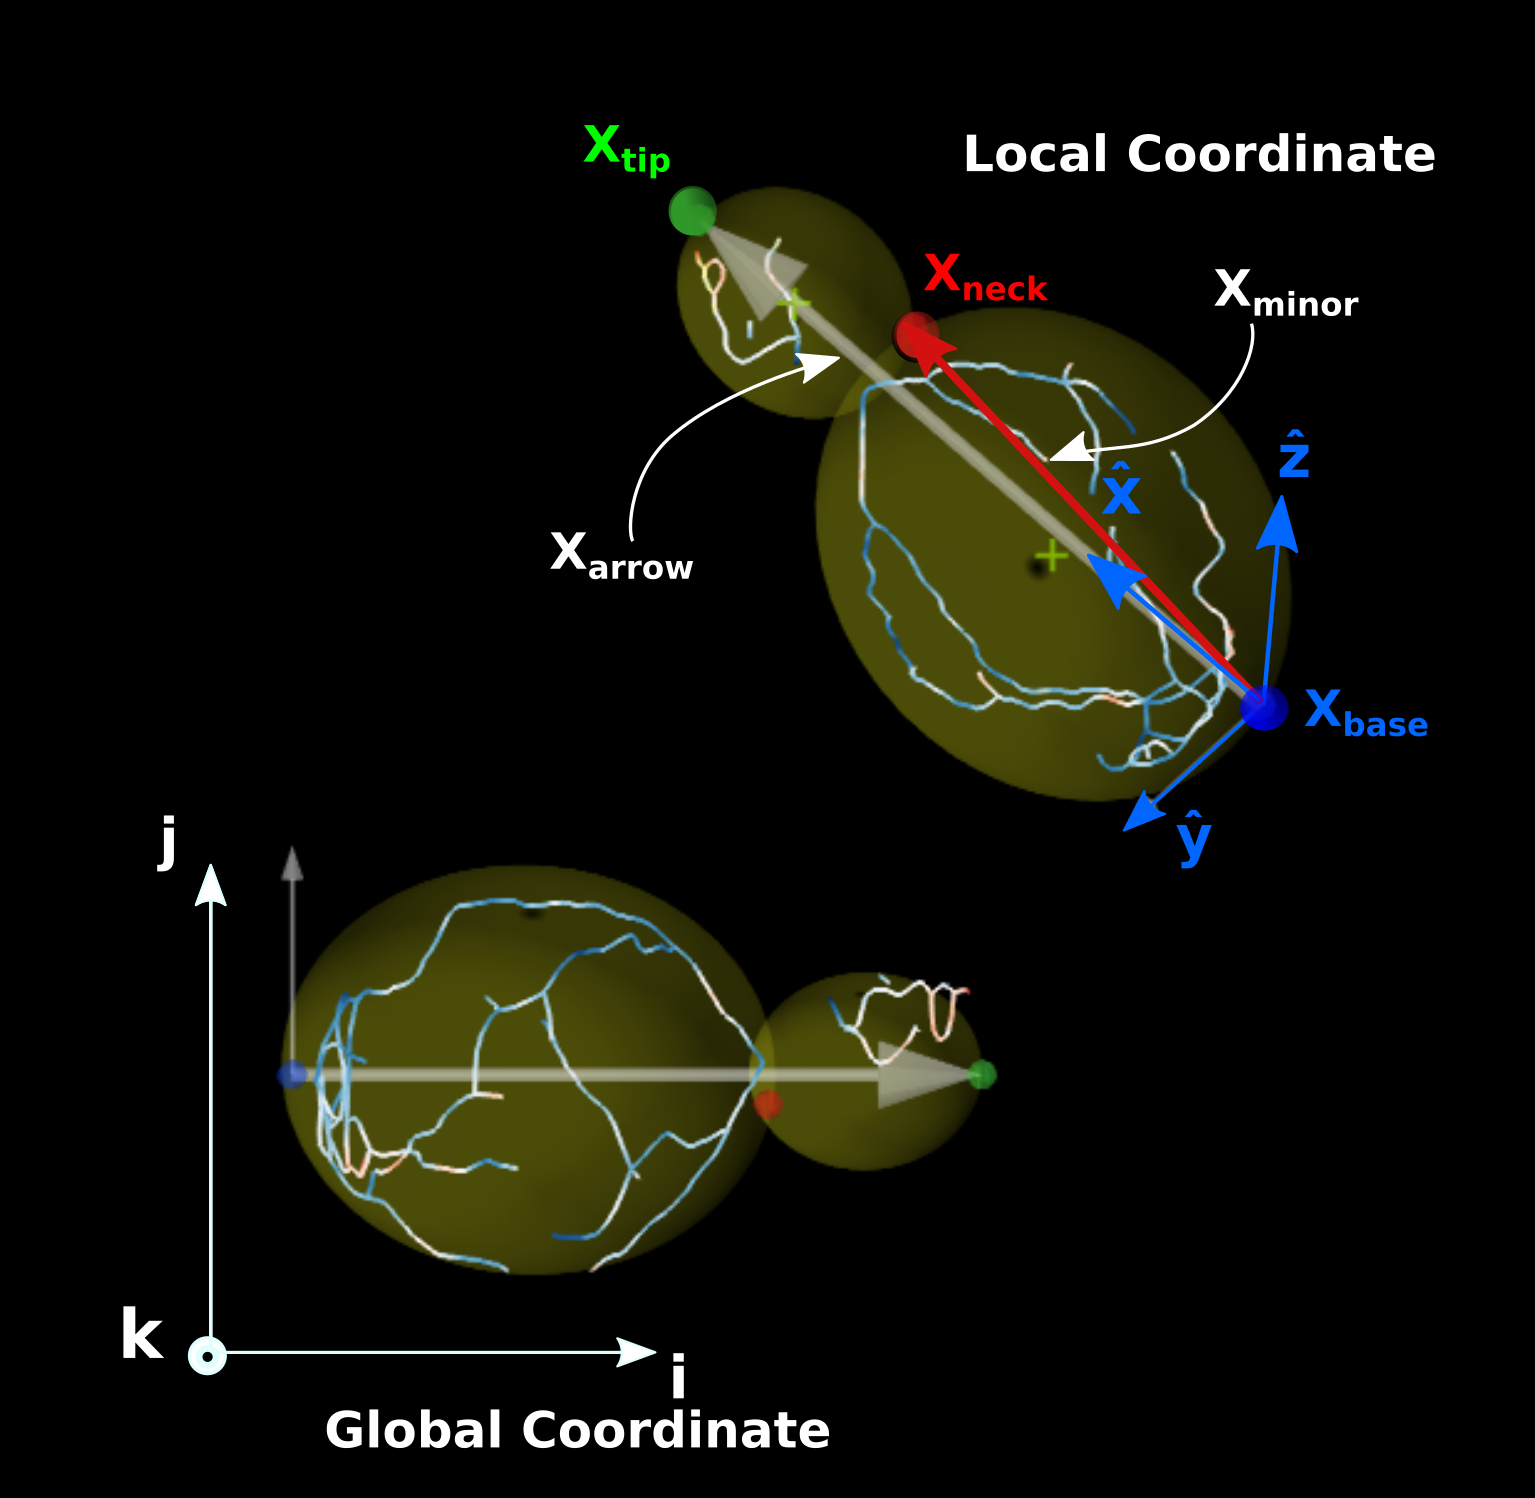
\includegraphics[width=.8\textwidth]{coors}
    \caption[Global and local coordinate system]{Global and local coordinate system.\\Shown in this figure is a mitochondrial network and cell that will be transformed from its original orientation in the 'Local Coordinate' to the 'Global Coordinate' system based on the Cartesian coordinate system with origin at $(0,0,0)$. The yellow ellipse surfaces represent the cortical periphery of the cell, with a mother (larger ellipse) and bud (smaller ellipse). The large arrow ($\mathbf{X_{arrow}}$) represents the mother-bud cell axis. A mouse callback routine written in Mayavi/Python was used to transform the cell by picking three points (blue,red and green). The blue and green points define the orientation of  $\mathbf{X_{arrow}}$. In order to constrain the rotation plane, a third point was needed and is represented by the red point. The location of the red point was chosen as the intersection between the mother and bud cell surfaces. The red arrow represents a position vector for this intersection (called the bud neck) and is coplanar with the $x-y$ plane of the local coordinate system. The transformation matrix translates and rotates the entire skeleton/cell so that the local $x-y$ plane lies on the global $x-y$ plane. The translation is based on the location of the blue point ( $\mathbf{X_{base}}$) so that after transformation the blue point lies on the origin $(0,0,0)$ of the global coordinate system.}\label{fig:coors}
\end{figure}
% 
%
\begin{figure}[htp]
	\centering
    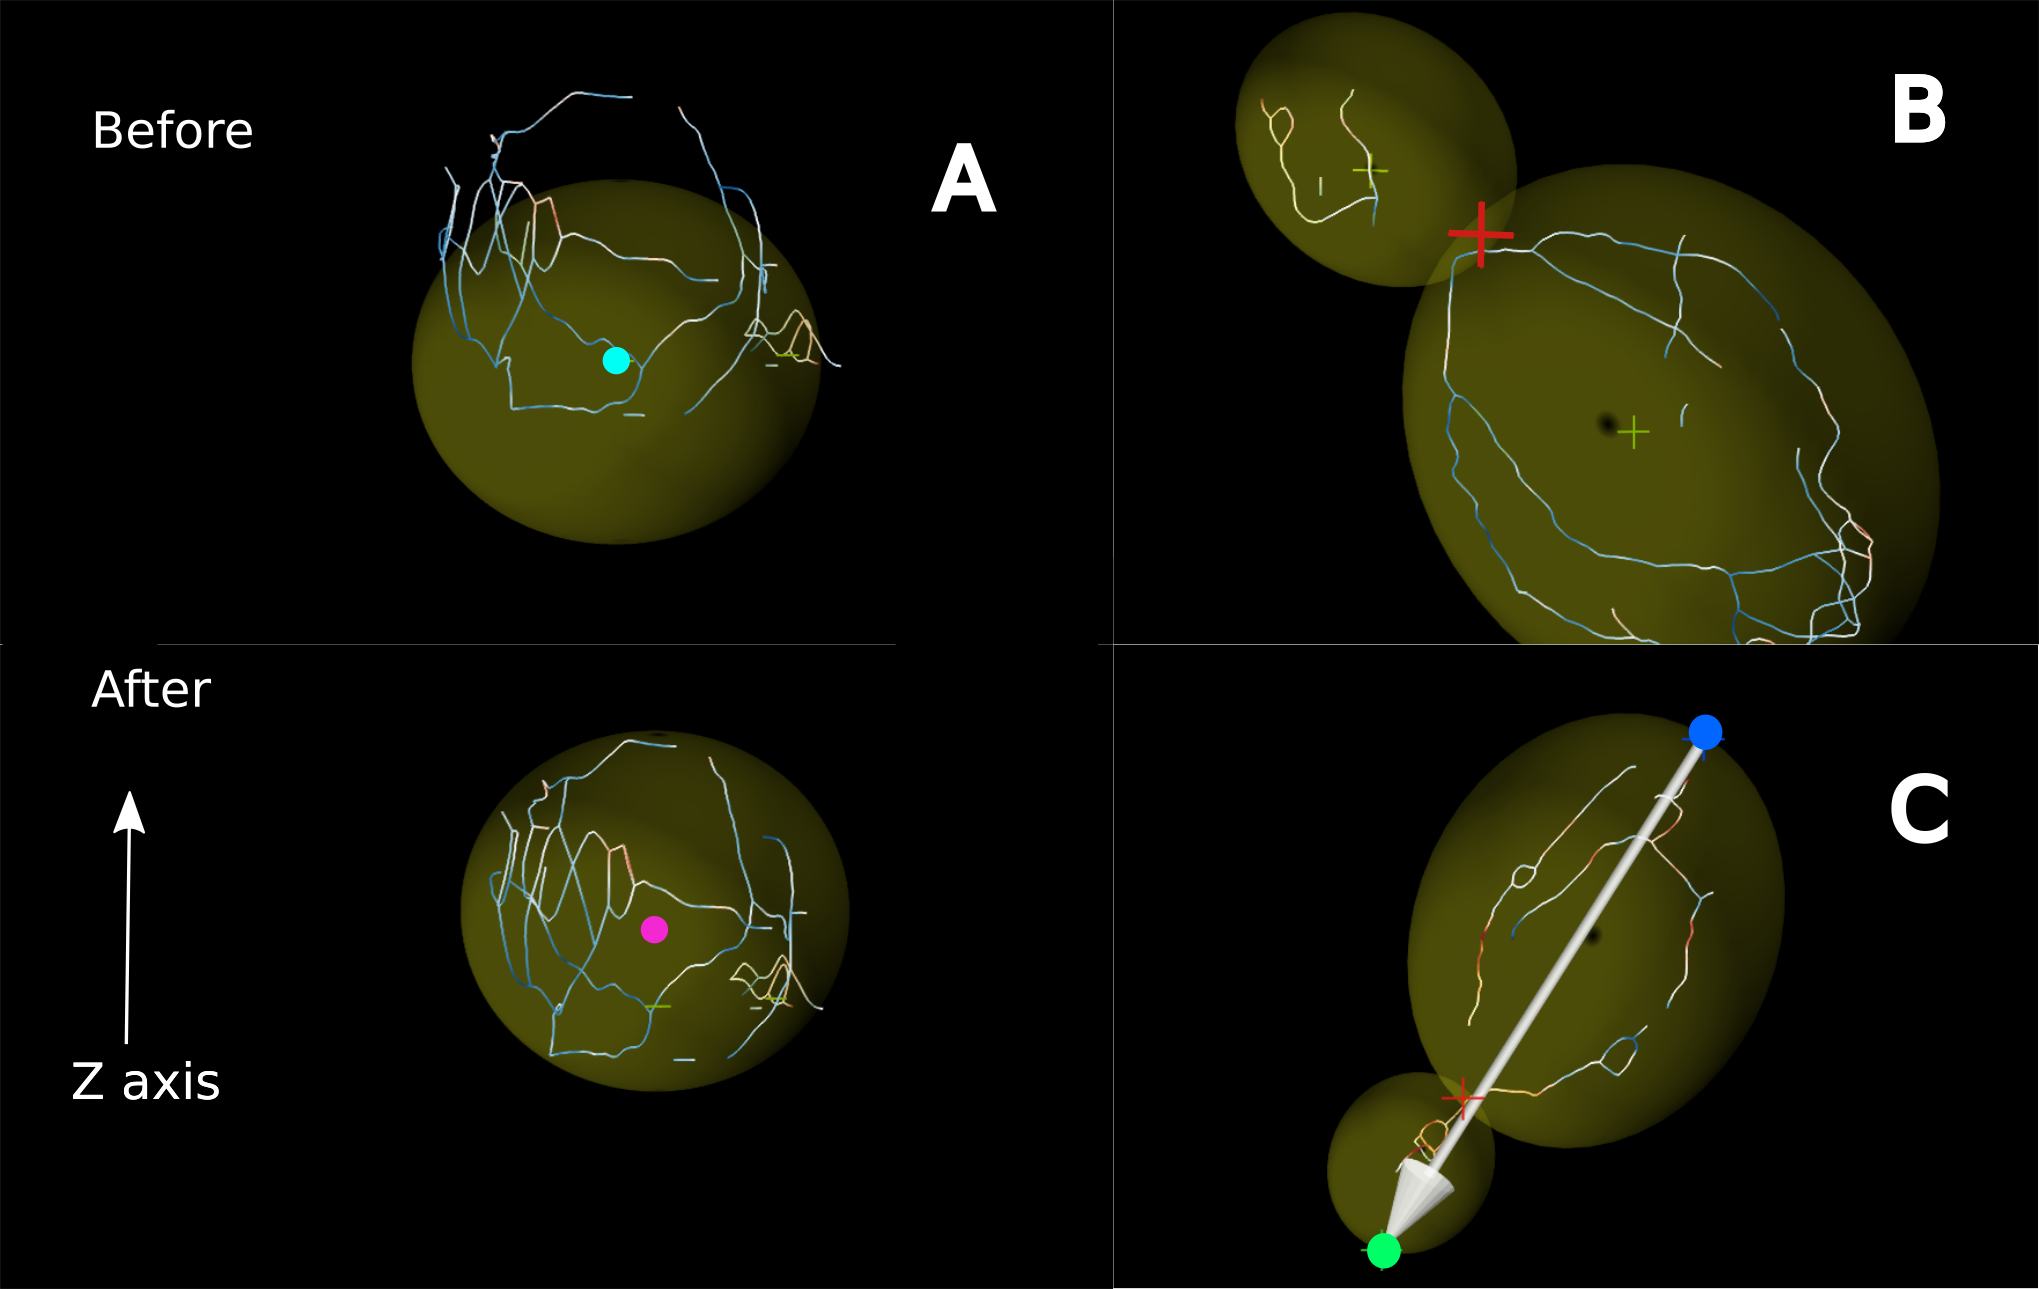
\includegraphics[width=.9\textwidth]{caveat}
     \subcaptionbox{An example of a skeleton that is not aligned with the cell surface (represented by the yellow ellipse, with the ellipse center shown in cyan). The cell surface was based on an ellipse fit of a hand traced outline of the inflection point in the $z-$position of the original brightfield image. The inflection point is the frame with the least visible outline of the cells in the brightfield image stack. A mouse callback function was used to pick the magenta point which repositions the cell surface so that it had good alignment with the skeleton.\label{fig:caveatA}}[\linewidth]{}
      \subcaptionbox{The bud neck region was picked based on the intersection of the two cell surfaces and is represented by the red cross. The bud neck coordinate is used to partition the cell into a mother and bud region.\label{fig:caveatB}}[\linewidth]{}
       \subcaptionbox{Care was always taken to pick the boundary of the cell based on the cortical periphery of the cell surface and not the skeleton. In this case the blue and green points were chosen to represent the base (blue) and tip (green) of the mother-bud cell axis.\label{fig:caveatC}}[\linewidth]{}
    \caption{Caveats when picking transformation points.}\label{fig:caveat}
\end{figure}
%
\subsection{Direction cosine based transformation matrix to realign the mother-bud cellular axis}
In order to analyze mother-bud functional asymmetry, it is necessary to define a coordinate system that conveniently aligns with the mother-bud cell axis. 
The direction cosine matrix is a matrix containing the cosines of the angle between a vector and its basis. It is used to express a vector in one orthogonal basis to a different basis \cite{kane_spacecraft_1983}. It can be used to transform the coordinates of all points in the mitochondrial skeleton so that for example, the mother-bud axis aligns parallel with the $x-$axis unit vector $(1\Vi+0\Vj+0\Vk)$. The transformation matrix $\mathbf{T}$ is given by:
\begin{equation}
	\begin{split}
		\begin{aligned}
			\mathbf{X_{global}} &= \mathbf{T X_{local}} \\
			%
			\mathbf{X_{global}} &= \text{vector coordinates expressed with basis } \mathbf{i,j,k} \\[-1.5ex]
			&\qquad\text{of the Cartesian coordinate system} \\
			%
			\mathbf{X_{local}} &= \text{vector coordinates expressed with basis } \mathbf{x,y,z} \\[-1.5ex]
			&\qquad\text{of the Cartesian coordinate system} 
		\end{aligned}
	\end{split}
\end{equation}
Suppose we want to transform the coordinates of all the points in the skeleton in \Fref{fig:coors} ('Local coordinate'). To define the mother-bud axis we pick two points represented by the blue and green dots. The blue and green dots represent the base and tip respectively of the mother-bud cell periphery. The mother-bud axis will be the main axis, and for convenience we define it as the $x-$axis of the local coordinate system. We need to pick another point to fix the plane of rotation, which we define as the plane formed by the blue (base), green (tip) and red (neck) dots and call this plane the $x-y$ plane in the local coordinate system. Therefore the three dots can be expressed as position vectors in the Cartesian coordinate system:
\begin{equation}
\begin{split}
		\begin{aligned}
		   \mathbf{X_{base}}&=X_{base}\Vi+Y_{base}\Vj+Z_{base}\Vk\\
		   \mathbf{X_{tip}}&=X_{tip}\Vi+Y_{tip}\Vj+Z_{tip}\Vk\\
		   \mathbf{X_{neck}}&=X_{neck}\Vi+Y_{neck}\Vj+Z_{neck}\Vk\\
		\end{aligned}
	\end{split}
\end{equation}
Consider a vector $\mathbf{X_{arrow}}$ represented by the large, white arrow in \Fref{fig:coors} ('Local coordinate') which represents the mother-bud axis. In the local coordinate system it has unit vectors $\xhat,\yhat,\zhat$:
\begin{equation}\label{eq:TM}
 	\begin{split}
	 	\begin{aligned}
	 		\mathbf{T}&=\begin{bmatrix}
			 		x_{1} &x_{2}&x_{3}&X_{base}\\
			 		y_{1} &y_{2}&y_{3}&Y_{base}\\
			 		z_{1} &z_{2}&z_{3}&Z_{base}\\
			 		0&0&0&1
		 		\end{bmatrix}		\\
		 	x_{1}, y_{1}, z_{1}\text{ are the direction } &\text{cosines of the x-axis in the local coord. system}\\[-1.5ex]
			x_{2}, y_{2}, z_{2}\text{ are the direction } &\text{cosines of the y-axis in the local coord. system}\\[-1.5ex]
			x_{3}, y_{3}, z_{3}\text{ are the direction } &\text{cosines of the z-axis in the local coord. system}
		\end{aligned}
	\end{split}
\end{equation}
The matrix formed by the direction cosines in \eqref{eq:TM} is the rotation matrix to rotate from the Cartesian to the local coordinate system, and the last column vector represents a translation from the origin $(0,0,0)$ to the position at $\mathbf{X_{base}}$.
The $(x_1, y_1, z_1)$ direction cosines of the vector $\mathbf{X_{arrow}}$, which has unit vector $\xhat$ is:
\begin{equation}\label{eq:dcosine}
	x_{1}= \frac{X_{tip}-X_{base}} {|X_{arrow}|} \quad x_{2}= \frac{Y_{tip}-Y_{base}} {|X_{arrow}|} \quad x_{3}= \frac{Z_{tip}-Z_{base}} {|X_{arrow}|}
\end{equation}
The direction cosines $(t_1, t_2, t_3)$ for $\mathbf{X_{minor}}$ can be found in the same manner as in equation \eqref{eq:dcosine} by replacing $\mathbf{X_{tip}}$ with $\mathbf{X_{neck}}$. 
Now, because the vectors $\mathbf{X_{arrow}}$ and $\mathbf{X_{minor}}$ (red arrow in \Fref{fig:coors}) formed by the three coplanar points $\mathbf{X_{base}}$, $\mathbf{X_{neck}}$ and $\mathbf{X_{tip}}$  lie on the $x-y$ plane of the local coordinate system, the unit vector $\zhat$ is orthogonal to this $x-y$ plane (i.e. the dot product of the vectors is zero):
\begin{align}
\mathbf{\hat{z_{base}}}\cdot \mathbf{X_{arrow}} &= x_3x_1+y_3y_1+z_3z_1=0 \nonumber \\
\mathbf{\hat{z_{base}}}\cdot \mathbf{X_{minor}} &= x_3t_1+x_3t_2+z_3t_3=0
\end{align}
Expressing $x_3$ and $y_3$ in terms of $z_3$ and using the unit vector definition of $\mathbf{Z_{base}}$ we obtain the $(x_3, y_3, z_3)$ components of the unit vector $\zhat$:
\begin{equation}
 	\begin{split}
	 	\begin{aligned}
	 		\zhat &= \frac {x_3\Vi+y_3\Vj+z_3\Vk}{\sqrt{x_3^2+y_3^3+z_3^2}}\\[1ex]
	 		\zhat &= \frac{x_3}{D}\Vi+\frac{y_3}{D}\Vj+\frac{z_3}{D}\Vk \\[1ex]
	 		\text{where D}&= \sqrt{\left(\frac{t_3}{t_1+t_2}\right)^2 +\left( \frac{t_3 x_1-t_1 z_1-t_2 z_1}{t_1 y_1+t_2 y_2}\right)^2+1}
		\end{aligned}
	\end{split}
\end{equation}	 	
Then obtaining the $(x_2, y_2, z_2)$ components of the unit vector $\yhat$ is done by taking the cross product of the other two orthogonal unit vectors:
\begin{equation}
\yhat=\zhat\times\xhat
\end{equation}
The transformation matrix to transform the cell so that the mother-bud axis is parallel to the Cartesian x-axis is just the inverse of $\mathbf{T}$. The inverse of the rotation matrix is its transpose. Therefore to align the arrow vector (which in our case, is the mother-bud axis) to be parallel to the unit vector $(1\Vi+0\Vj+0\Vk)$ the transformation matrix is:
\begin{equation}
		\mathbf{T^{-1}}=\begin{bmatrix}
			 		x_{1} &y_{1}&z_{1}& -X_{base}\\
			 		x_{2} &y_{2}&z_{2}&-Y_{base}\\
			 		x_{3} &y_{3}&z_{3}& -Z_{base}\\
			 		0&0&0&1
		 		\end{bmatrix}		
	\end{equation}

We used the math functions in VTK to obtain the cross product and set the transformation matrix $\mathbf{T^{-1}}$ as a filter to be applied to the original skeleton. This results in a skeleton transformed and aligned as shown in \Fref{fig:coors} ('Global coordinate').

The source code for transforming the cell is included in Appendix \ref{mbcode}.
\subsection{Tracking functional heterogeneity during budding progression}\label{sec:cellcycle}
Once the skeleton was transformed so that the mother-bud axis was aligned with global Cartesian $x-$axis, we partitioned the cell into a 'mother' and 'bud' region by comparing the $x-$coordinates of all points in the skeleton to the 'neck' point. Points lower than the neck point value were classified as belonging to the mother region while those greater were classified as a bud region. We tracked budding progression using the volume of the bud. Buds have relatively stable mitochondrial content and cell size, in contrast to their mothers that grow larger and show reduced mitochondrial volume ratio as they age \cite{rafelski_mitochondrial_2012}. We defined the bud to have completed cell division when it reached a volume that was equal to the largest 10\% of buds.
\section{Results}
\subsection{Buds have mitochondria with higher ΔΨ compared to mother cells}\label{sec:frady}
Previous studies have shown that mother cells accumulate more damaged cellular components such as oxidized proteins and impaired mitochondria \cite{aguilaniu_asymmetric_2003,lai_mutation_2002,laun_aged_2001}. We find similar results in our dataset of budding yeasts grown in various carbon sources representing different respiratory conditions (see \fref{sec:carbon} for details). Since we are comparing intracellular ΔΨ heterogeneity when comparing mother and buds, we scaled the ΔΨ values of each cell so that its min and max values correspond to 0 and 1 respectively. In all conditions buds have a statistically higher average ΔΨ compared to their mothers (\Fref{fig:mbviol}, statistical testing done as in \fref{sec:stat} with the test function modified to a Wilcoxon signed rank test for paired samples).
 
We also expressed the heterogeneity of mother-bud ΔΨ as a ratio between the mean ΔΨ of the bud to the mean ΔΨ of the mother for each cell. A ratio greater than one means the bud has an average ΔΨ greater than the mother. The distributions of this ratio across the different respiratory conditions are shown in \Fref{fig:fraviol}. On average buds have a median ΔΨ that was 20\% greater than the mother. There was no statistical difference in the mean ΔΨ bud/ΔΨ mother ratio across all groups except for glycerol+ethanol (statistical testing done as in \fref{sec:stat}), indicating that buds had a higher ΔΨ than their mothers. However not all cells had buds with ΔΨ larger than their mothers; on average 65\% of cells had buds with a larger ΔΨ compared to their mothers. The mother-bud ΔΨ asymmetry was smallest in the glycerol+ethanol population, both in their magnitude and proportion of cells.
%
\begin{figure}[htp]
	\centering
    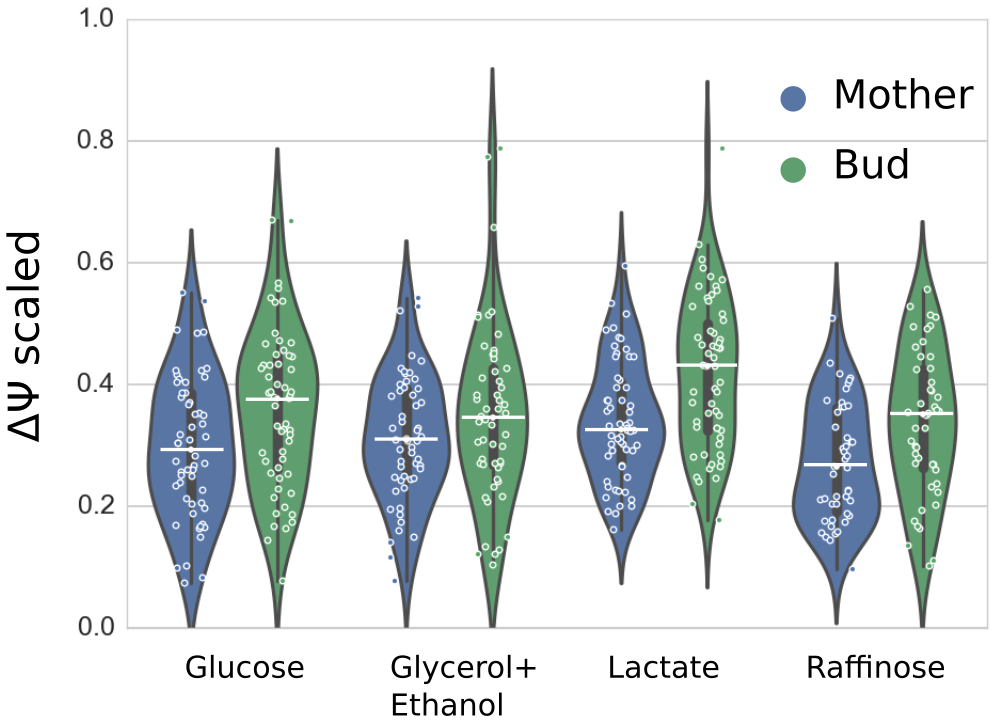
\includegraphics[width=.68\textwidth]{mbviol}
    \caption[Buds have higher mitochondrial membrane potential (ΔΨ) compared to their mothers]{Buds have higher mitochondrial membrane potential (ΔΨ) compared to their mothers.\\Shown in this figure is the distribution of the scaled ΔΨ distribution of all buds and mothers grown in different carbon sources. The scaled ΔΨ represents the mean ΔΨ value of a particular bud or mother scaled to the min and max ΔΨ value for that cell. Buds have a statistically significant higher ΔΨ compared to their mothers for all conditions ($p$<0.05 based on Wilcoxon signed rank test for paired samples, with post-hoc multiple testing correction).\\\emph{White bars indicate the median values for the scaled ΔΨ.\\Number of mother-bud pairs---Glucose=56, Glycerol+Ethanol=54, Lactate=58, Raffinose=46}}\label{fig:mbviol}
\end{figure}
%
%
\begin{figure}[htp]
	\centering
    \hspace*{1in}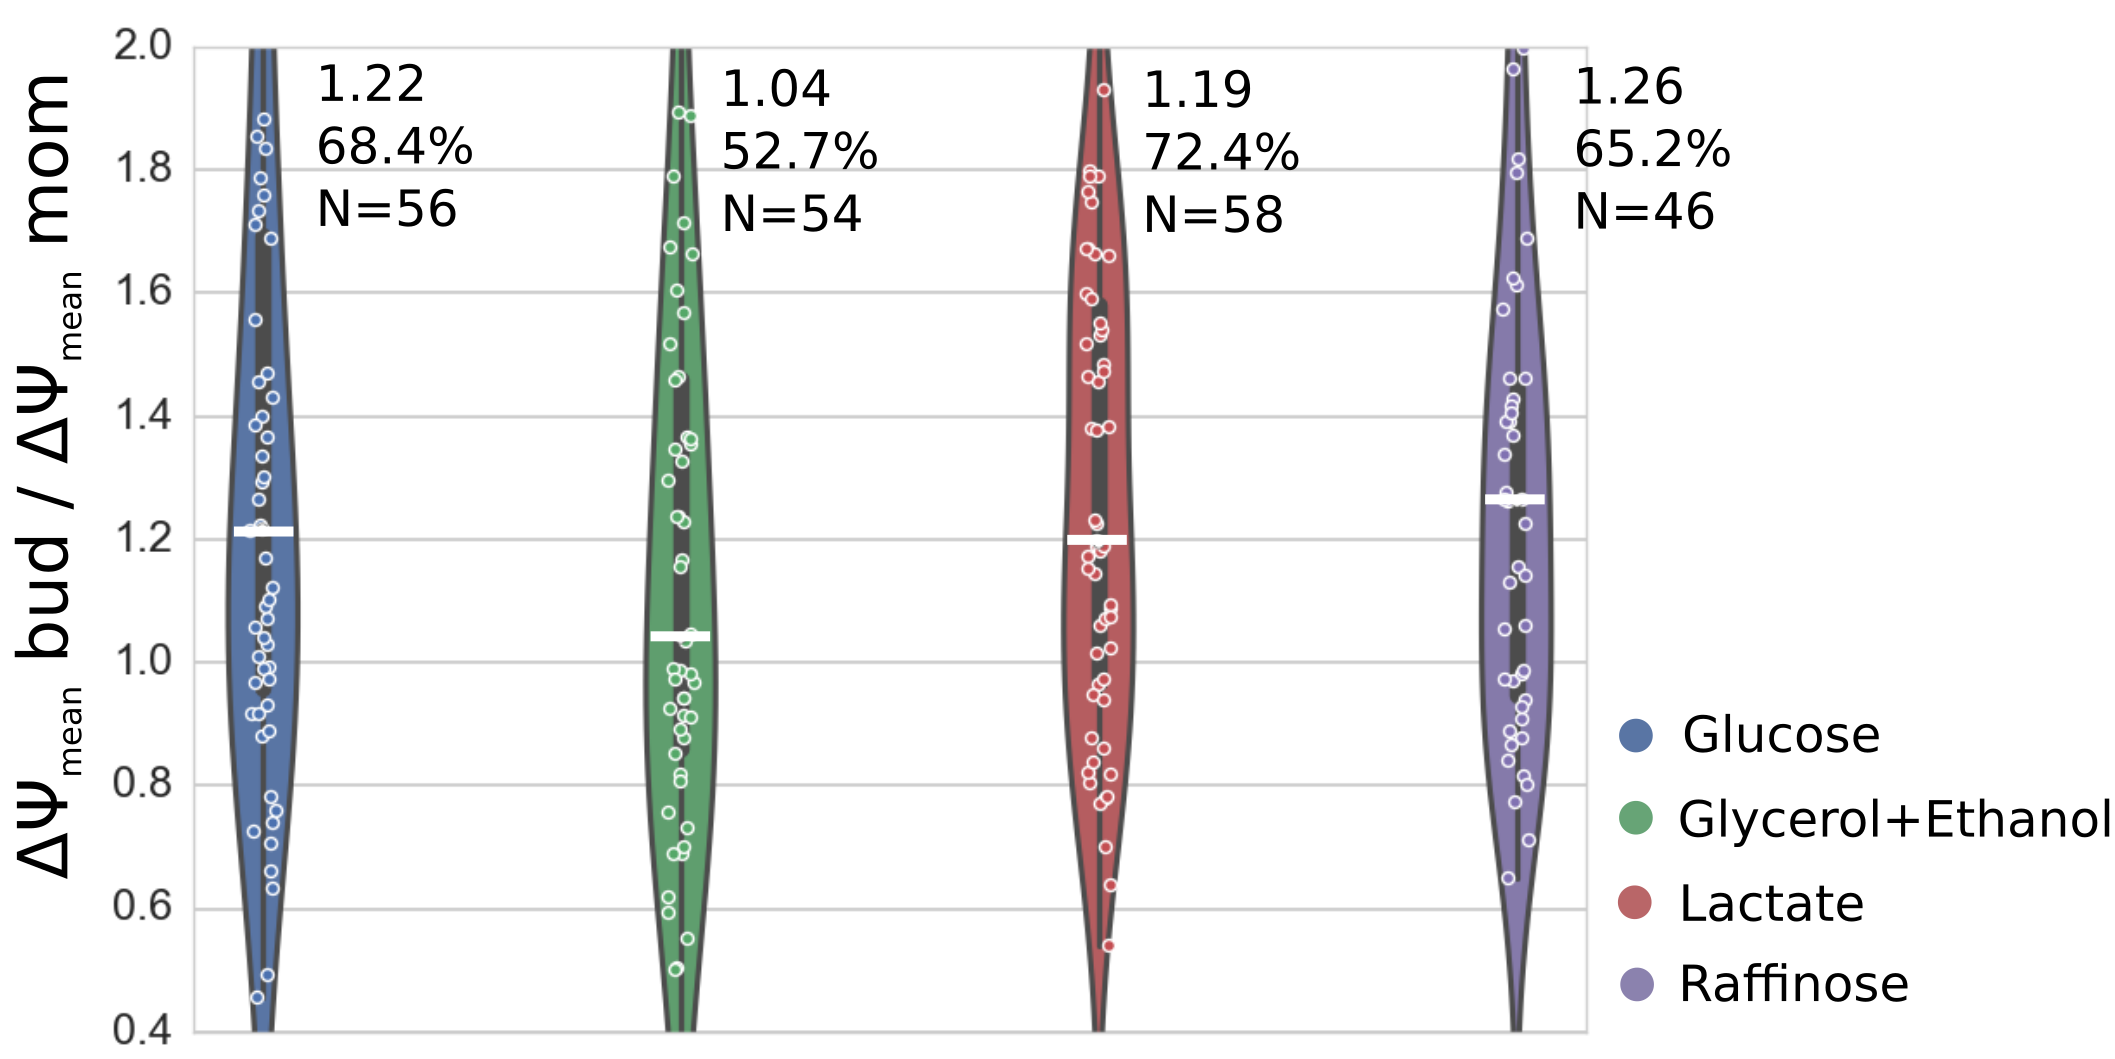
\includegraphics[width=.8\textwidth]{fraviol}
    \caption[Distribution of ΔΨ$_\mathrm{bud}/$ΔΨ$_\mathrm{mother}$ in different carbon sources]{Distribution of ΔΨ$_\mathrm{bud}/$ΔΨ$_\mathrm{mother}$ in different carbon sources.\\The ratio of ΔΨ$_\mathrm{bud}/$ΔΨ$_\mathrm{mother}$ was used to quantify the number of cells where the average ΔΨ of the bud was higher than the mother as well as the average magnitude of this ratio. The first row of numbers represent the average magnitude of ΔΨ$_\mathrm{bud}/$ΔΨ$_\mathrm{mother}$. The mean of this magnitude was about 1.2 (20\% higher ΔΨ in the bud). The second row of numbers represent the proportion of mother-bud pairs where the bud had a higher ΔΨ compared to the mother. The last row of numbers represent the number of mother-bud pairs for each population.\\\emph{White bars indicate the median values for the ratio of} ΔΨ$_\mathrm{bud}/$ΔΨ$_\mathrm{mother}$.}\label{fig:fraviol}
\end{figure}
%
\subsection{Mitochondria display different gradients of ΔΨ along the mother-bud axis}
To analyze the distribution of ΔΨ along the mother-bud cell axis, we partitioned cells into a mother and bud region and defined two separate coordinate systems (one for the mother and one for the bud, each scaled 0--1). The intersection point (bud neck) had a value of 1 for the mother and 0 for the bud in their respective coordinate systems. The corresponding plot for the mother regions for each carbon source is shown in \Fref{fig:aldymom}. For the bud regions, we further partitioned the plots according to bud volumes, as these represented different stages of bud growth. The partition bins are labeled as 'binvol' in \Fref{fig:aldybud}, representing bud volume in \si{\micron\cubed}). The ΔΨ values in these plots were scaled to the min and max of the entire cell axis (mother and bud) for each cell. We observe a pattern where ΔΨ was lowest at the mother distal end, gradually rises and plateaus halfway in the mother cell for the populations of glycerol+ethanol, lactate and raffinose (\Fref{fig:aldymom}). For glucose,  ΔΨ does not seem to plateau but appears to continue to rise, although the error bars are large enough that a plateau cannot be ruled out.
%
\begin{figure}[htp]
	\centering
    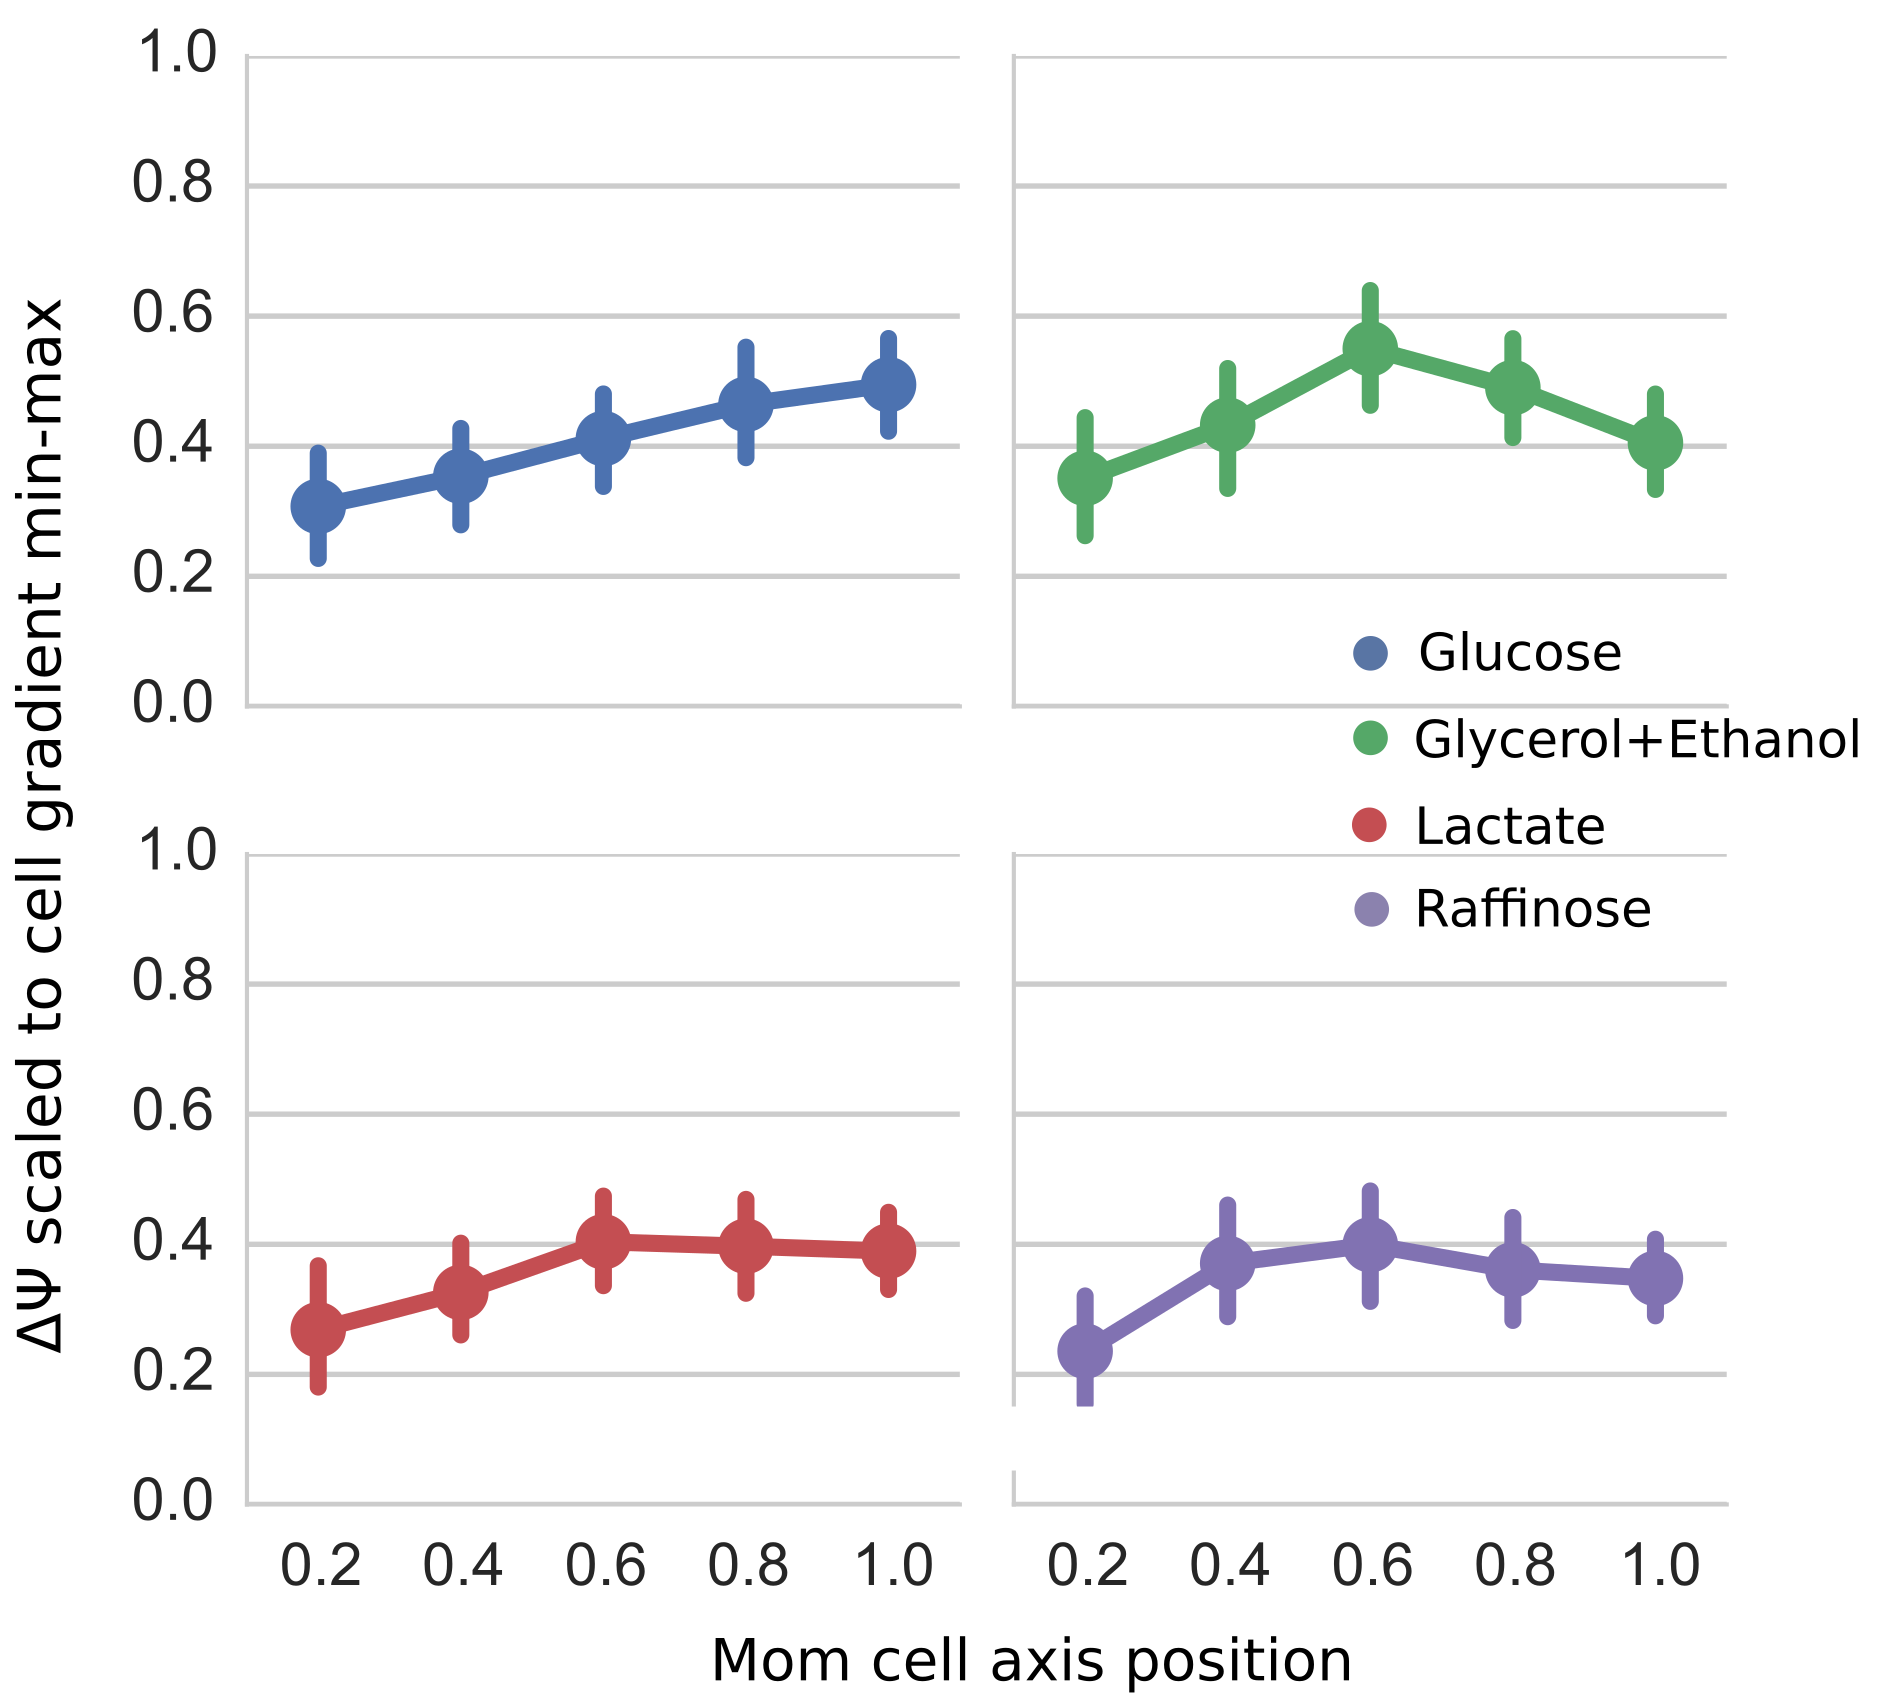
\includegraphics[width=.52\textwidth]{aldymom}
    \caption[Spatial distribution of ΔΨ along the mother cell axis]{Spatial distribution of ΔΨ along the mother cell axis.\\Shown in this figures is a plot of the average ΔΨ at each position along the mother axis (position 0 is at the mother distal end away from the bud neck, position 1 is at the bud neck). ΔΨ gradually increases from the mother distal end and plateaus halfway along the axis.\\\emph{Error bars represent the 95\% confidence interval of the median ΔΨ at each position along the mother cell axis.\\Number of cells---Glucose=56, Glycerol+Ethanol=54, Lactate=58, Raffinose=46}}\label{fig:aldymom}
\end{figure}
%

It was harder to discern a clear pattern for the progression of ΔΨ in buds (\Fref{fig:aldybud}). Due to partitioning the buds into different bud volumes, the sample numbers were reduced for each bud volume category and hence the error bars were larger compared to the mother plots. It appears that larger buds have a more consistent/flat ΔΨ distribution compared to smaller buds, except for the case of raffinose. Consistent with the results from \Fref{sec:frady}, the bud region displays a higher average ΔΨ compared to the mother regions. There appears to be a discontinuity (i.e. a sudden rise in ΔΨ) at the bud neck region when moving from the mother to the bud. 
%
\begin{figure}[htp]
	\centering
    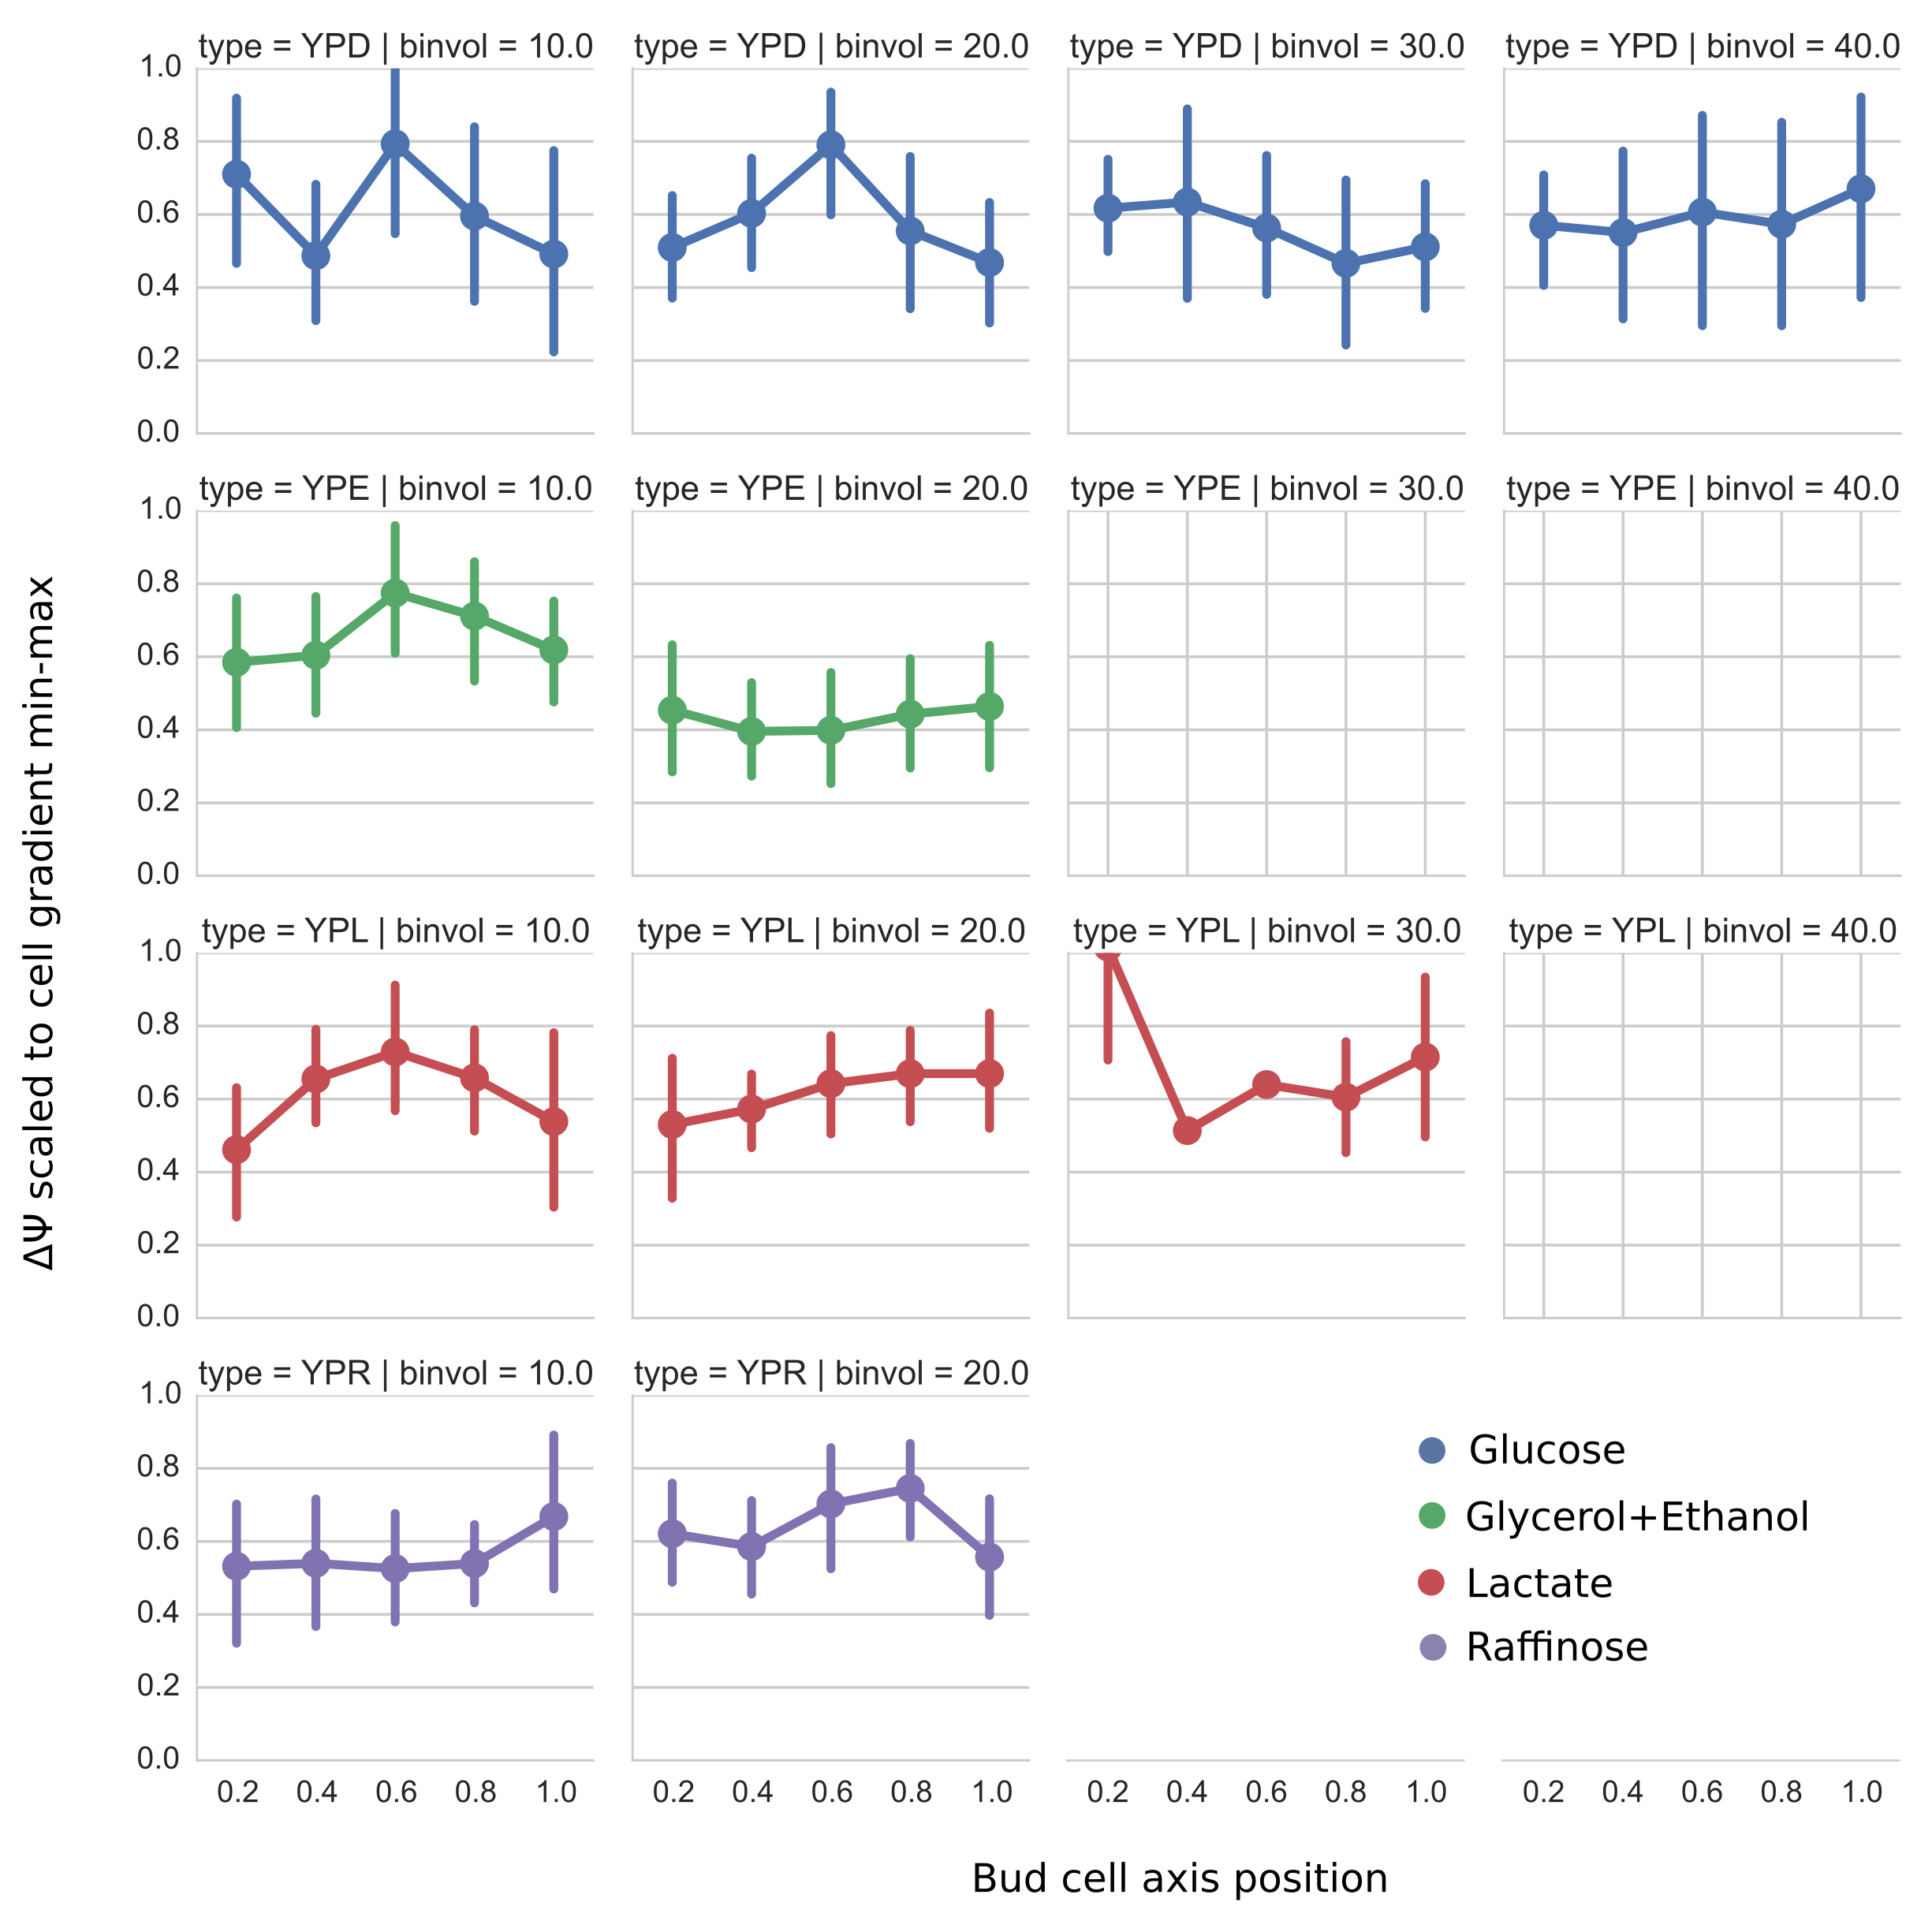
\includegraphics[width=.8\textwidth]{aldybud}
    \caption[Spatial distribution of ΔΨ along the bud cell axis]{Spatial distribution of ΔΨ along the bud cell axis.\\Shown in this figures is a plot of the average ΔΨ at each position along the bud axis (position 0 is at the the bud neck, position 1 is at bud end opposite the bud neck). The buds are partitioned according to their volume. The partitioning bins are labeled as 'binvol', representing bud volume in \si{\micron\cubed}). Larger buds display a more consistent/flat ΔΨ distribution compared to smaller buds, except for the case of raffinose.\\\emph{Error bars represent the 95\% confidence interval of the median ΔΨ at each position along the bud cell axis.\\Number of cells---Glucose=56, Glycerol+Ethanol=54, Lactate=58, Raffinose=46}}\label{fig:aldybud}
\end{figure}
%
\subsection{Mitochondrial ΔΨ asymmetry is maintained during the budding progression}
We tracked the ratio of bud ΔΨ to mother ΔΨ as a function of budding progression (defined in \Fref{sec:cellcycle}) to see if there was a change in the functional asymmetry of ΔΨ as budding progressed. As shown in \Fref{fig:frabud}, with the exception of glycerol+ethanol this ratio is maintained above 1 throughout budding progression. This indicates that mitochondrial bud quality is maintained at a higher level throughout the cell cycle. Glycerol+ethanol grown cells display a reduction in this ratio to values below 1 at intermediate values of bud volume. We found that while glycerol+ethanol had the lowest bud ΔΨ to mother ΔΨ ratio, for most of the budding progression it was above 1. We also partitioned the the data in \Fref{fig:frabud} according to bud volumes, similar to what was done for the bud ΔΨ gradient in \Fref{fig:aldybud}. As shown in \Fref{fig:frafacet}, there does not appear to be an obvious change in the ΔΨ asymmetry between cells with smaller and larger buds.
%
\begin{figure}[htp]
	\centering
    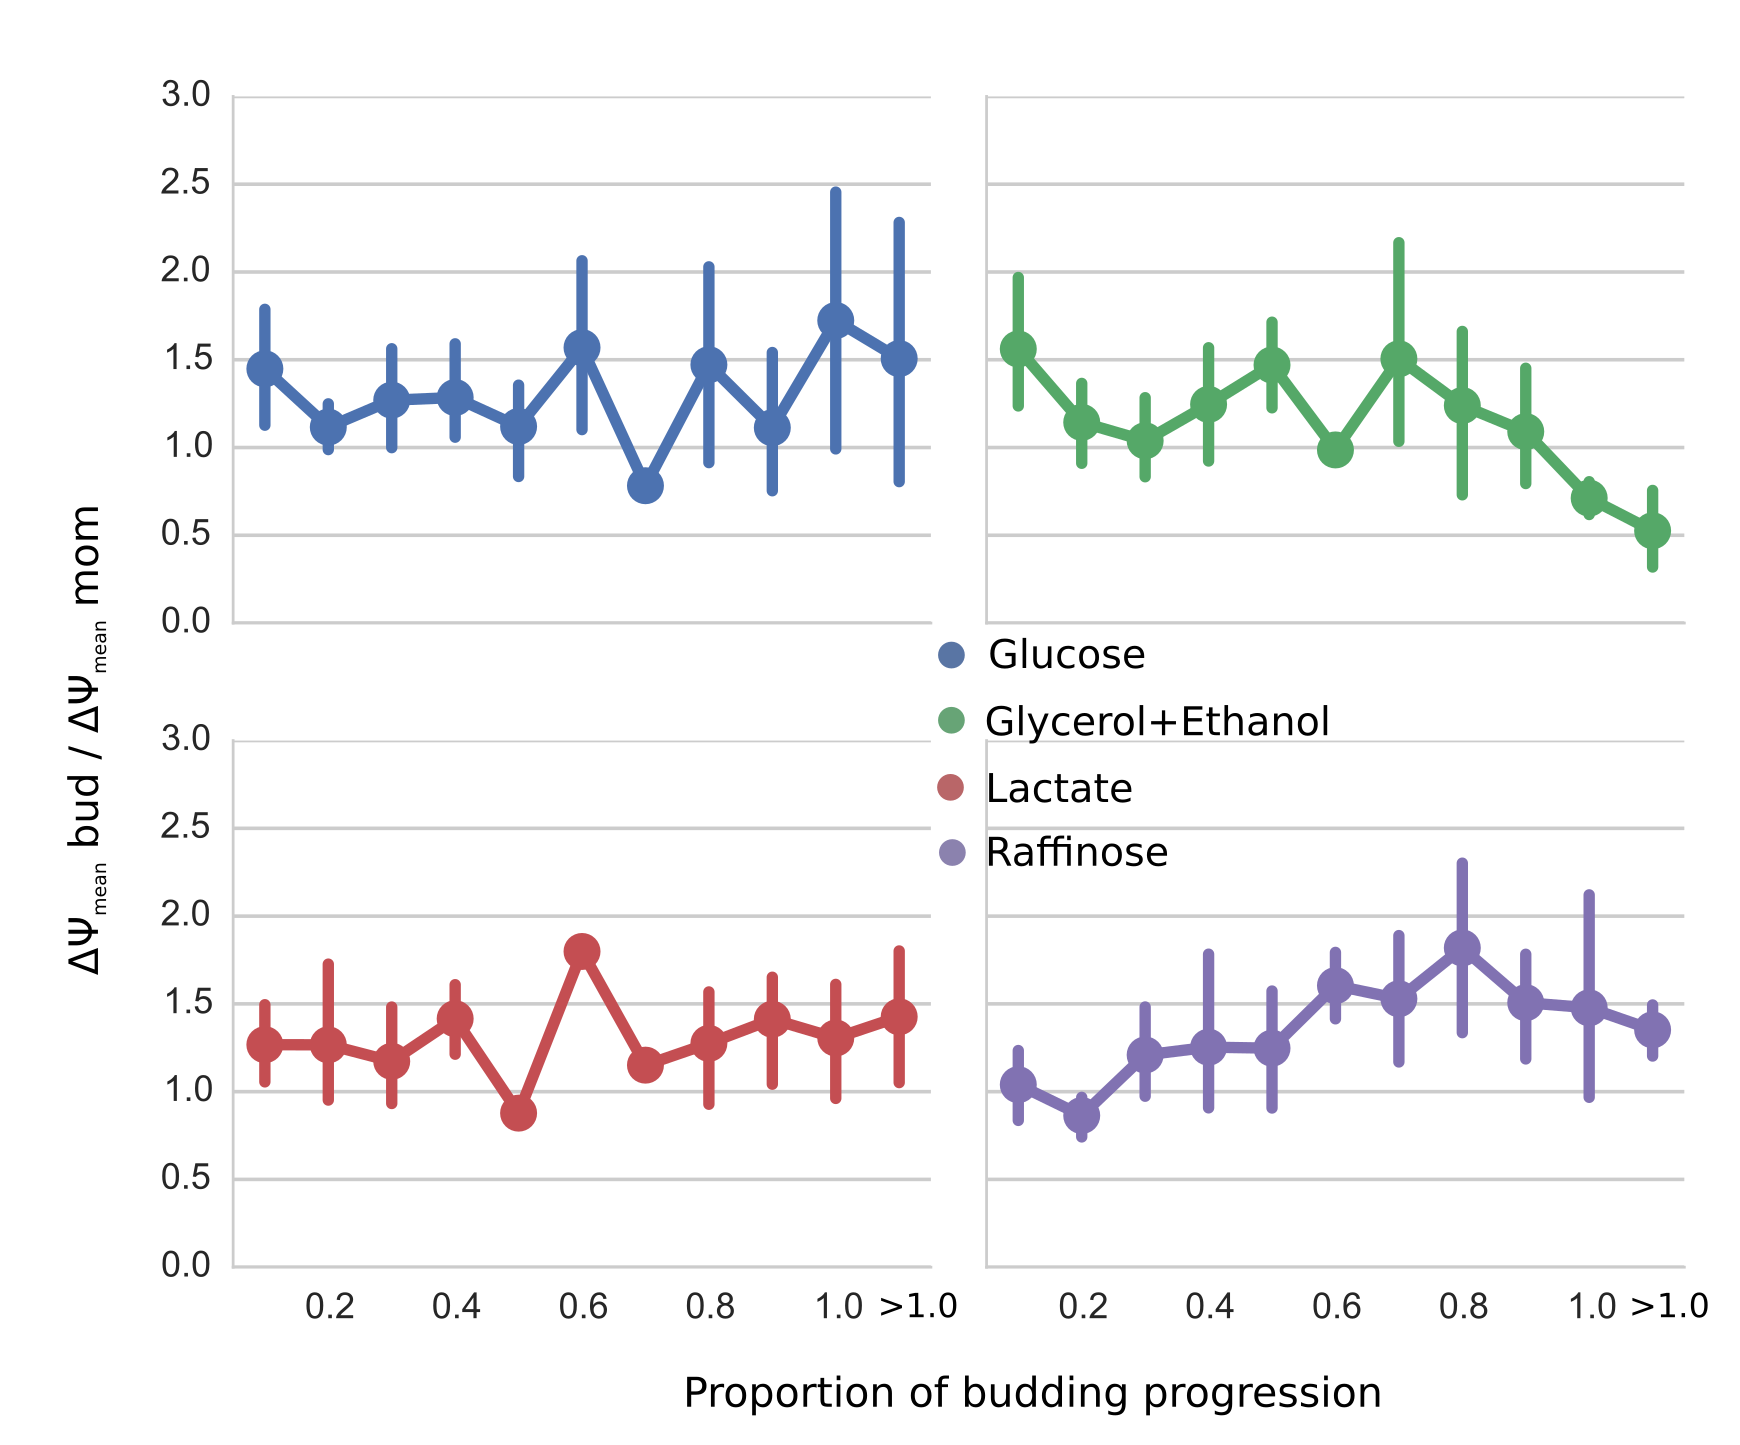
\includegraphics[width=.75\textwidth]{frabud}
    \caption[Mitochondrial ΔΨ asymmetry is maintained throughout the cell cycle]{Mitochondrial ΔΨ asymmetry is maintained throughout the cell cycle.\\The ΔΨ$_\mathrm{bud}/$ΔΨ$_\mathrm{mother}$ ratio for each cell was plotted as a function of budding progression. There was no significant difference in this ratio as we moved from early in the cell cycle to completion of cell division. This indicates that the mitochondrial ΔΨ asymmetry is maintained throughout the cell cycle.\\\emph{Error bars represent the 95\% confidence interval of the median ΔΨ$_\mathrm{bud}/$ΔΨ$_\mathrm{mother}$ ratio at each value for budding progression.\\Number of cells---Glucose=56, Glycerol+Ethanol=54, Lactate=58, Raffinose=46}}\label{fig:frabud}
\end{figure}
%
%
\begin{figure}[htp]
	\centering
    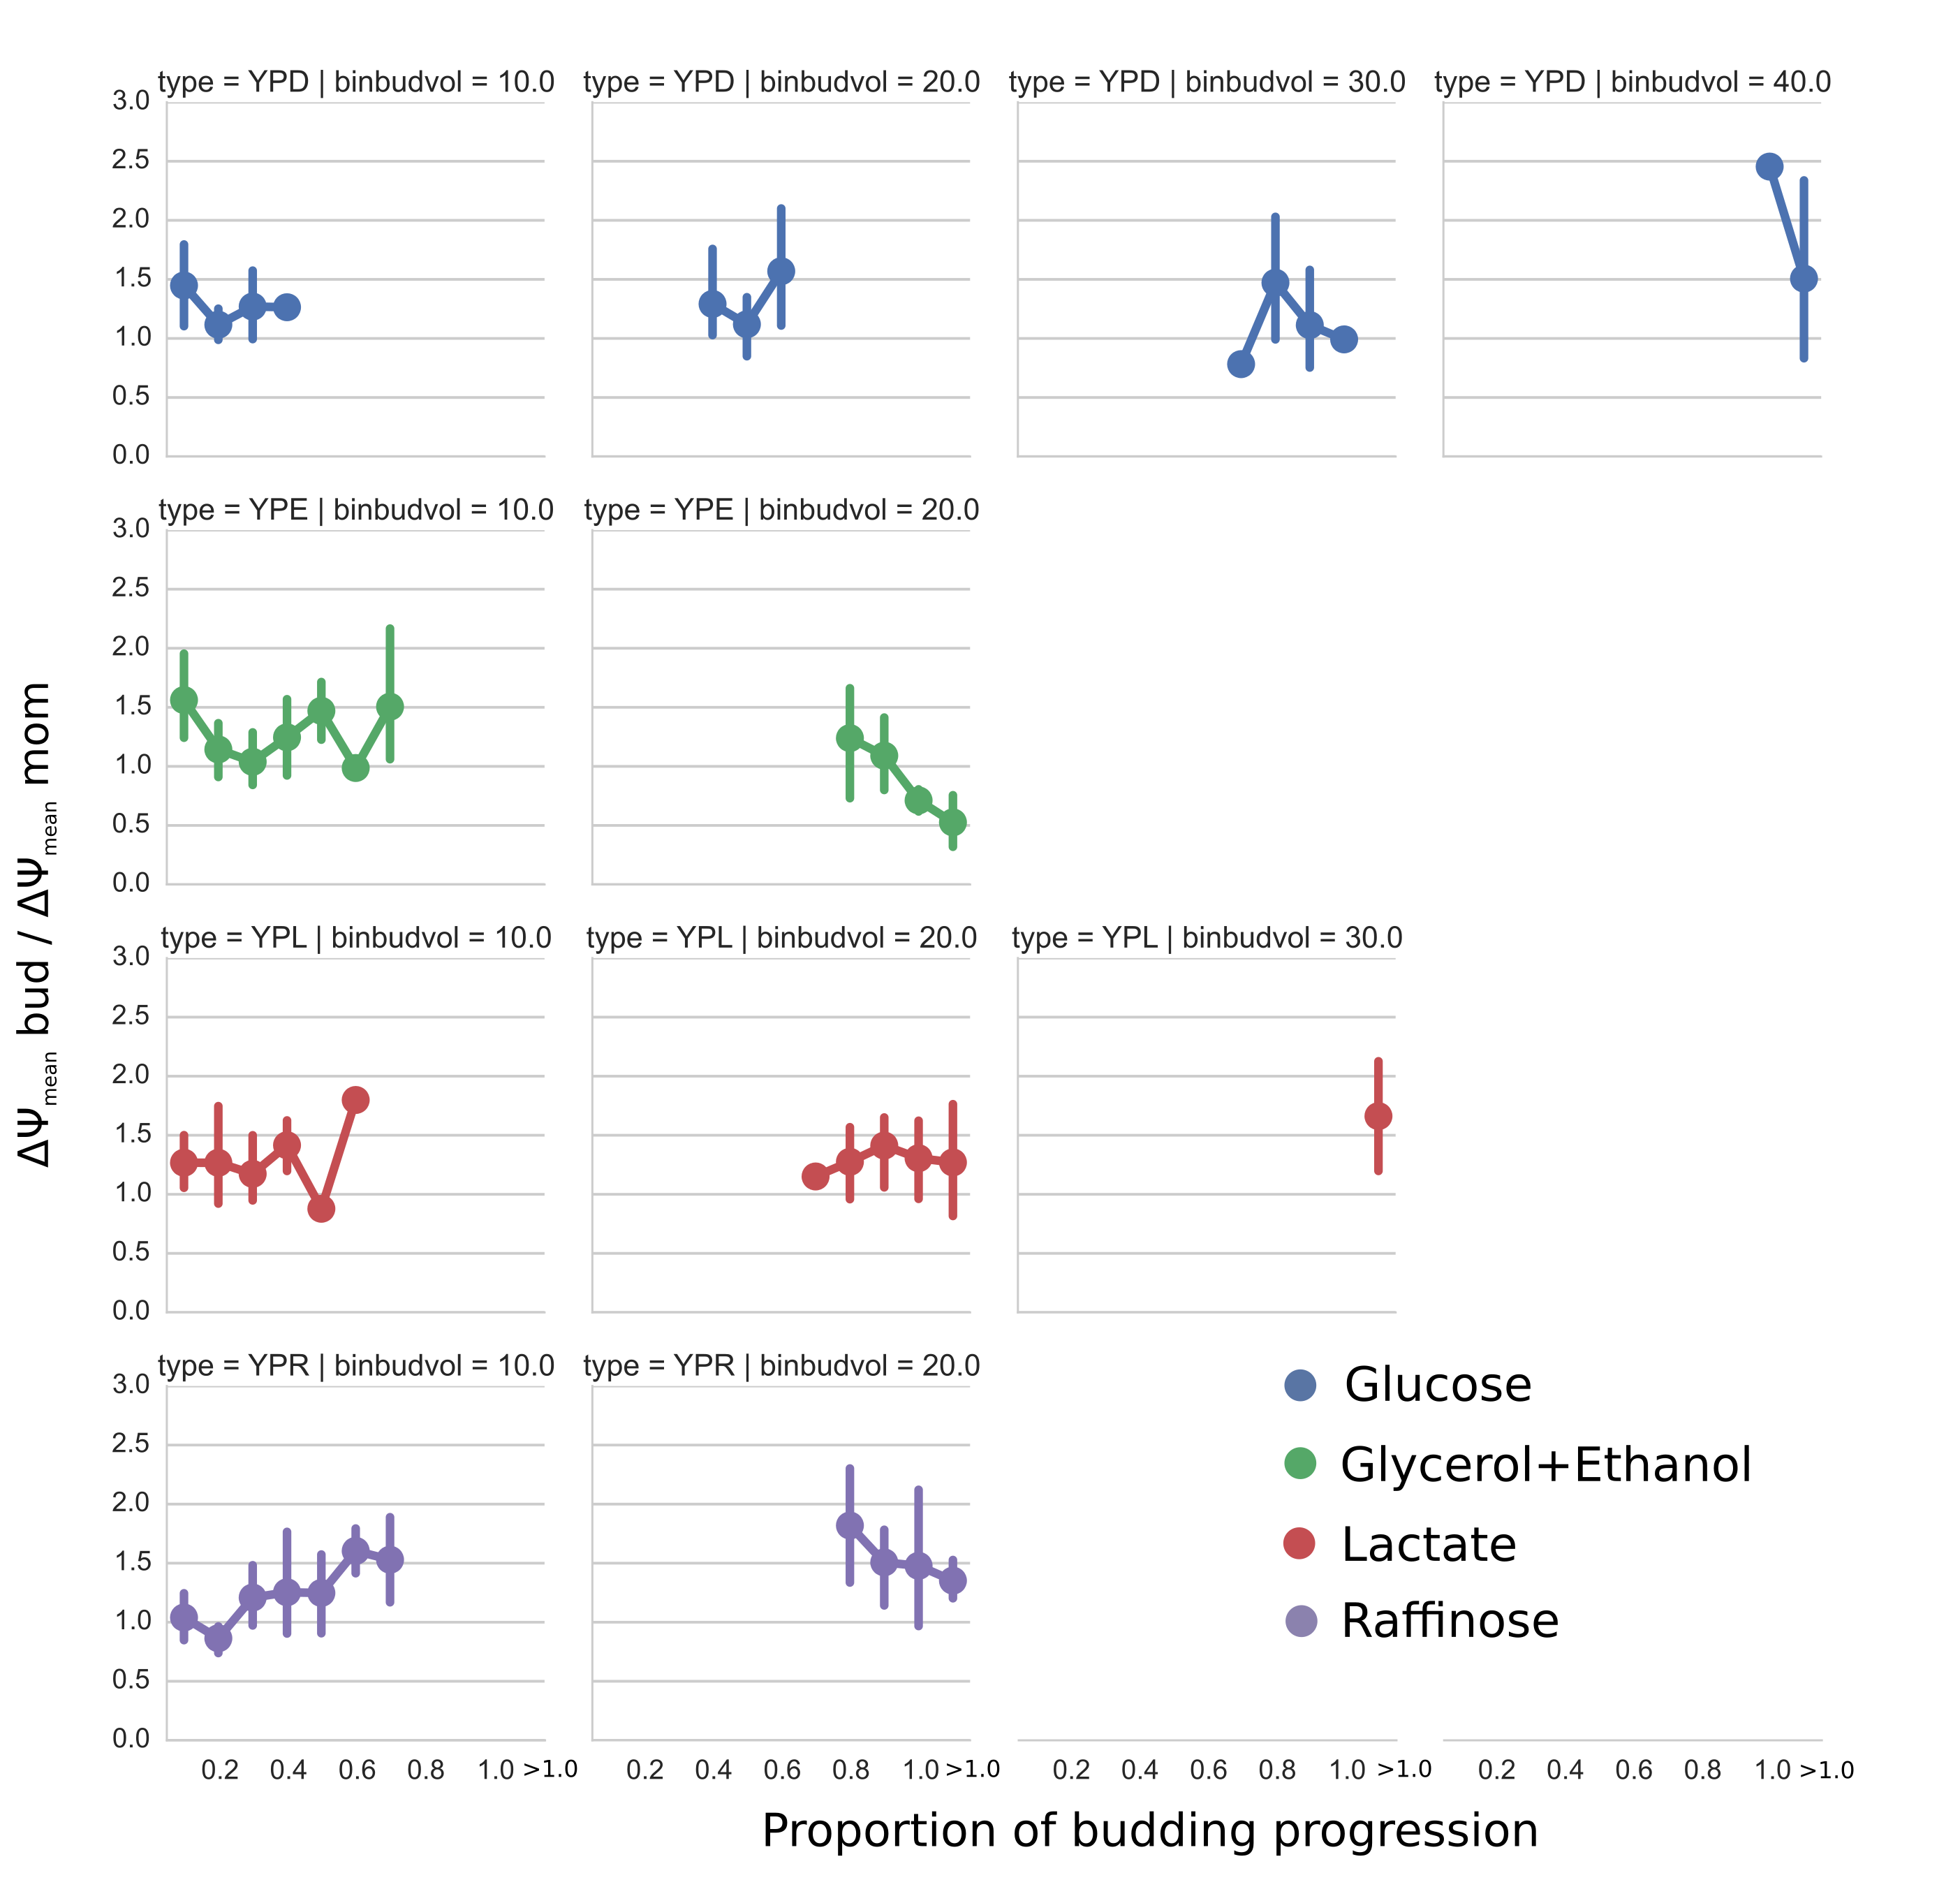
\includegraphics[width=.8\textwidth]{frafacet}
    \caption[Bud size has no effect on mitochondrial ΔΨ asymmetry in the cell]{Bud size has no effect on mitochondrial ΔΨ asymmetry in the cell.\\ ΔΨ$_\mathrm{bud}/$ΔΨ$_\mathrm{mother}$ ratio as a function of budding progression was plotted at different partitions of bud volumes. The partitioning bins are labeled as 'binvol', representing bud volume in \si{\micron\cubed}). There was no significant difference in ΔΨ asymmetry between cells with smaller and larger buds.}\label{fig:frafacet}
\end{figure}
%
\section{Discussion}
We have analyzed and confirmed that mitochondrial networks in yeast display an asymmetry of mitochondrial quality between mother and daughter cells (buds), similar to previously reported results. Our results were obtained after careful segmentation of the mother-bud axis in three dimensions as detailed in this chapter. We found that this asymmetry exists regardless of whether the cell was undergoing fermentation or aerobic respiration. This suggests that yeast preserve the machinery to preferentially distribute higher quality mitochondria to their buds even when respiration demand of the cell is low. This suggests that the distribution of mitochondria with higher levels of ΔΨ to the progeny (bud) is inherently essential not just for aerobic respiration but perhaps for other functions that are ΔΨ dependent, such as mitochondrial fusion and mitochondrial protein import \cite{dudek_mitochondrial_2013}. Our results also suggest that ΔΨ asymmetry persists throughout the entire budding progression cycle. This suggest that ΔΨ asymmetry results from a segregation mechanism that is active throughout the cell division cycle.
 
Our results showing a gradient of ΔΨ in the mother cell that plateaus halfway towards the bud is interesting as it suggests a possible mitochondrial quality segregation process occuring at the distal end of the mother cell. We speculate that the mechanism for this segregation process involves some sort of preferential retention of lower quality mitochondria at the distal end of the mother cell. Mitochondria are tethered at the mother end by a mitochondrial-ER-cortex-anchor (MECA) complex \cite{lackner2013endoplasmic}). This complex is absent from small buds and is localized to larger buds and mother cells. At least two proteins, Num1 and Mdm36 are essential components of this tethering complex. Thus one way to test our hypothesis on segregation of mitochondria at the mother distal end is to disrupt the expression of NUM1 or MDM36 to see if the ΔΨ gradient in the mother is altered or even abolished.

Our result showing a discontinuity and sudden increase in ΔΨ at the bud neck suggest another 'hurdle' or quality threshold that mitochondria must overcome to enter the bud. Another possibility is that the anchorage machinery at the bud tip preferentially binds to higher quality mitochondria. The Myo2 myosin has been implicated in transporting mitochondria across the bud neck \cite{fortsch2011myosin}. In addition, Mmr1 and Ypt11 are proteins that have been identified as having a role in binding mitochondria to Myo2. Recent studies indicate that mitochondria are tethered to the bud tip via interactions with the cortical ER (cER). Anchorage of mitochondria to cER has been shown to be dependent on Mmr1 \cite{swayne_role_2011}. Thus one way to investigate the mechanism of mitochondrial quality selection at the bud is to disrupt or modulate the expression of MYO2, MMR1 and YPT11 with a β-estradiol gene induction and protein degradation system \cite{mcisaac2011fast}. While there have been studies of functional asymmetry in mmr1Δ (for example in \cite{mcfaline-figueroa_mitochondrial_2011}), these have only focused on the differences in magnitude of ΔΨ asymmetry between mother and bud. Our method allows us to study how the spatial distribution of asymmetry and the discontinuity of ΔΨ at the bud neck is affected by deletion or modulation of MYO2, MMR1 and YPT11. Such an analysis provides a possible mechanistic insight into how the mitochondrial inheritance machinery plays a role in mitochondrial quality selection during cell division.

Interestingly we found that the magnitude of ΔΨ asymmetry between mother and bud was smallest in the glycerol+ethanol cells (\Fref{fig:fraviol}). We showed in \Fref{ch:three} that cells grown in glycerol+ethanol had the highest average ΔΨ. Perhaps this indicates that that there is a limit to the ΔΨ level that buds can inherit. Since glycerol+ethanol population has the highest overall ΔΨ compared to the other populations, a bud inheriting mitochondria with similar ΔΨ asymmetry levels as the other populations would have excessively high ΔΨ.

In conclusion, we have shown that the distribution of ΔΨ along the mother-bud axis displays some interesting features which put quantitative restrictions on any future mathematical models of how mitochondrial functional asymmetry is achieved. Our findings also suggests that the mitochondrial quality selection process involves the mitochondrial transport and tethering machinery. 
